\documentclass[11pt]{article}
\usepackage[margin=1in]{geometry}
\usepackage[T1]{fontenc}
\usepackage{lmodern}
\usepackage{microtype}
\usepackage{booktabs}
\usepackage{amsmath}
\usepackage{listings}
\usepackage{xcolor}
\usepackage{pgfplots}
\pgfplotsset{compat=1.18}
\usepackage[numbers,sort&compress]{natbib}
\usepackage[hidelinks]{hyperref}

\lstset{basicstyle=\ttfamily\small,columns=fullflexible,frame=single,
  framerule=0.3pt,rulecolor=\color{black!30},breaklines=true,
  keywordstyle=\bfseries,showstringspaces=false}

\title{dbcomparer: Engine-Agnostic Schema and Data Comparison\\for Relational Databases}
\author{Rakesh S Rai\\[2pt]
  \small Independent Researcher, USA\\
  \small ORCID: \href{https://orcid.org/0009-0009-5110-3230}{0009-0009-5110-3230}}
\date{November 2026}

\begin{document}
\maketitle

\begin{abstract}
Researchers and data engineers routinely need to show that two relational
databases hold the same data: before and after a schema migration, across
re-runs of an ETL pipeline, or between a production system and an archived
snapshot. Byte-level checksums cannot answer this question because physical
layout, type spelling and row order differ between engines and versions.
We present \texttt{dbcomparer}, an open-source Python package and
command-line tool that compares both the schema and the row-level contents
of any two databases reachable through SQLAlchemy, including databases on
\emph{different} engines such as PostgreSQL and SQLite. It normalises column
types to a generic vocabulary and values across database drivers, matches
rows by primary key or user-chosen keys, compares keyless tables as
multisets, and emits text, Markdown, JSON or HTML reports with exit codes
suited to continuous integration. On commodity hardware it compares one
million rows per side in about seven seconds (roughly 280{,}000 rows per
second), with the same throughput for a PostgreSQL--SQLite pair as for
SQLite--SQLite, and it recovers every injected difference exactly. The
software is MIT-licensed and archived at
\href{https://doi.org/10.5281/zenodo.24213702}{doi:10.5281/zenodo.24213702}.
\end{abstract}

\section{Introduction}

Relational databases hold much of the data behind scientific and
engineering work, including observation catalogues, laboratory information
systems, survey responses and simulation outputs \citep{codd1970relational}.
Guidance on reproducible research asks that derived data be verifiable
across software and infrastructure changes
\citep{sandve2013ten,wilson2014best,wilkinson2016fair}. For flat files this is
straightforward: a checksum or a textual \texttt{diff} suffices. For
databases it is not. Two databases holding identical information can differ
byte for byte because of page layout, physical row order, collation, type
spelling (\texttt{VARCHAR(20)} versus \texttt{TEXT}), or driver
representations of the same value (\texttt{Decimal('1.50')} versus
\texttt{1.5}). Conversely, real changes can hide in places a quick row
count does not reveal, such as a dropped \texttt{NOT NULL} constraint or a
single changed value.

Typical questions that arise in practice include:
\begin{itemize}
  \item Did a schema migration or ORM upgrade change any data?
  \item Does the SQLite snapshot deposited with a paper match the
        PostgreSQL database the analysis actually ran on?
  \item Did re-running an ETL pipeline with a new library version produce
        the same tables?
  \item Do two collaborators' copies of a shared database agree?
\end{itemize}

This paper describes \texttt{dbcomparer}, a small, dependency-light tool
that answers these questions for any pair of databases supported by
SQLAlchemy \citep{sqlalchemy}. It builds on the universal database
comparison framework of \citet{rai2026universal}, which normalises records
from heterogeneous database systems into a common representation;
\texttt{dbcomparer} provides an open, tested and installable implementation
of those ideas for SQL databases.

Our contributions are:
\begin{enumerate}
  \item a unified comparison of schema (tables, columns, types,
        nullability, primary keys, indexes, foreign keys) and data (rows
        added, removed and changed, with per-column before/after values);
  \item normalisation rules for types and values that make
        \emph{cross-engine} comparison practical without spurious
        differences;
  \item a single-pass, ordering-independent hash-join algorithm for row
        matching, with multiset semantics for tables without keys;
  \item an empirical evaluation of correctness and performance on SQLite
        and PostgreSQL.
\end{enumerate}

\section{Related work}

\paragraph{Schema migration tools.} Alembic \citep{alembic} and
\texttt{migra} \citep{migra} compare a database schema against a model or
another database and generate migration scripts. They are designed to
\emph{change} schemas rather than to verify data, they do not compare row
contents, and \texttt{migra} supports PostgreSQL only.

\paragraph{Data diff tools.} \texttt{data-diff} \citep{datadiff} compared
tables within or across databases using checksums over key ranges, which
scales to very large warehouse tables by pushing hashing into the
database. Its open-source development has been archived, it requires each
engine to implement compatible hashing and ordering, and it reports data
differences only, without the schema context needed to interpret them.

\paragraph{Engine-specific utilities.} Vendor tools and dump-and-diff
workflows (e.g.\ comparing \texttt{pg\_dump} outputs) are tied to one
engine, are sensitive to dump ordering and formatting, and cannot compare
across engines.

\texttt{dbcomparer} occupies a gap between these: engine-agnostic, schema
and data together, with structured output intended to be stored alongside a
research record or asserted on in a test suite.

\section{Design}

\subsection{Architecture}

\texttt{dbcomparer} is organised into three layers: (i) a comparison core
(\texttt{compare\_schema}, \texttt{compare\_data} and the combined
\texttt{compare\_databases}) that accepts SQLAlchemy engines or connection
URLs; (ii) a result model of plain Python dataclasses that serialise
losslessly to JSON; and (iii) renderers and a command-line interface. The
core never issues engine-specific SQL: schema information comes from
SQLAlchemy's runtime inspector, and data is read with portable
\texttt{SELECT} statements. Supporting a new engine therefore requires only
an existing SQLAlchemy dialect.

\subsection{Schema comparison}

For each database the inspector lists tables (optionally filtered by glob
patterns and a schema namespace). Tables present on only one side are
reported as added or removed. For tables on both sides we compare:

\begin{itemize}
  \item \textbf{Columns}: presence, type and nullability.
  \item \textbf{Primary key}: the ordered list of key columns.
  \item \textbf{Indexes}: a signature consisting of uniqueness and column
        list (index \emph{names} are ignored, as they are frequently
        auto-generated and differ between engines).
  \item \textbf{Foreign keys}: a signature of constrained columns, referred
        table and referred columns.
\end{itemize}

\paragraph{Type normalisation.} By default each reflected type is mapped
to its generic SQLAlchemy type via \texttt{as\_generic()}, so that, for
example, PostgreSQL \texttt{CHARACTER VARYING(20)} and SQLite
\texttt{VARCHAR(10)} both become \texttt{STRING}. A \emph{strict} mode
compares the compiled, dialect-specific type instead, for cases where
lengths and precisions matter.

\paragraph{Nullability normalisation.} Primary-key columns are
\texttt{NOT NULL} by definition in standard SQL, but SQLite reports
\texttt{INTEGER PRIMARY KEY} columns as nullable. Without correction this
yields a spurious difference in every PostgreSQL--SQLite comparison; our
cross-engine tests detected exactly this, and \texttt{dbcomparer} now
treats key columns as non-nullable on both sides.

\subsection{Data comparison}

\paragraph{Row identity.} Rows are matched on a key: the table's primary
key by default, or columns supplied by the user per table. Only columns
present on both sides are compared, and the user may exclude volatile
columns such as \texttt{updated\_at}.

\paragraph{Algorithm.} A naive approach would issue \texttt{ORDER BY key}
on both sides and merge the two sorted streams. This is fragile across
engines because sort order depends on collation, \texttt{NULL} placement
and type coercion, which differ between engines. \texttt{dbcomparer}
instead performs an order-independent hash join
\citep{graefe1993query}:

\begin{enumerate}
  \item Stream the source table in chunks (default 10{,}000 rows) and
        insert each row into a hash map keyed by its normalised key.
  \item Stream the target table. For each row, look up and remove its key
        from the map. If absent, record the row as \emph{added}; if
        present with different normalised non-key values, record it as
        \emph{changed}, keeping per-column source and target values.
  \item Rows left in the map are \emph{removed}.
\end{enumerate}

This reads each table once, sequentially, needs no ordering guarantees,
and runs in $O(n_s + n_t)$ time and $O(n_s)$ memory. Counts are always
exact; to keep reports readable the number of example rows recorded per
category is capped (default 100, configurable).

\paragraph{Keyless tables.} Tables without any key cannot be matched
row-by-row, but they can still be compared as multisets: we count
occurrences of each normalised row on both sides and report the multiset
differences. This correctly detects, for example, a duplicated row that
became unique.

\paragraph{Value normalisation.} Before comparison, values are normalised
so that representations of the same datum from different drivers compare
equal: \texttt{Decimal} and \texttt{float} are unified; booleans are
mapped to integers (SQLite has no boolean type); binary values are
hex-encoded; time-zone-aware timestamps are converted to UTC; and
\texttt{NaN} compares equal to \texttt{NaN}. An optional absolute float
tolerance $\varepsilon$ quantises floating-point values to multiples of
$\varepsilon$ before comparison, which suppresses round-off differences
introduced by format conversions.

\subsection{Interfaces}

The command-line interface takes two SQLAlchemy URLs:

\begin{lstlisting}[language=bash]
dbcomparer postgresql://user@host/prod sqlite:///snapshot.db \
    --key measurements=station_id,ts --ignore-column updated_at \
    --float-tolerance 1e-9 --format markdown -o report.md
\end{lstlisting}

It exits with status 0 if the databases are equivalent, 1 if differences
were found and 2 on error, so it can gate a CI job directly. The same
functionality is available from Python:

\begin{lstlisting}[language=Python]
from dbcomparer import compare_databases
from dbcomparer.report import to_json

res = compare_databases("sqlite:///before.db", "sqlite:///after.db",
                        keys={"measurements": ["station_id", "ts"]})
assert not res.has_differences, to_json(res)
\end{lstlisting}

\section{Evaluation}

\subsection{Correctness}

The test suite (18 tests, 95\% line coverage) exercises each category of
schema and data difference, keyless multiset comparison, custom keys,
ignored columns, float tolerance, report truncation, generic versus strict
type matching, every report format and the CLI exit codes. A separate
cross-engine test loads identical data containing integer, string,
fixed-point and boolean columns into PostgreSQL~16 and SQLite and asserts
that no difference is reported, then modifies one value and asserts that
exactly that row is reported as changed. Continuous integration runs the
suite on Linux, macOS and Windows with Python 3.9, 3.11 and 3.13.

\subsection{Performance}

\paragraph{Setup.} The benchmark script (\texttt{benchmarks/run.py} in the
repository) builds a table \texttt{obs} with columns \texttt{id} (\texttt{BIGINT}
primary key), \texttt{station} (\texttt{INT}), \texttt{value}
(\texttt{DOUBLE}), \texttt{label} (\texttt{VARCHAR(32)}) and \texttt{ts}
(\texttt{TIMESTAMP}), holding $N$ rows of
pseudo-random data, and a target copy in which 1\% of rows differ: 0.5\%
changed, 0.25\% removed and 0.25\% added. We measure wall-clock time of
\texttt{compare\_data} and peak resident memory, each in a fresh process,
taking the median of three runs. Runs used a 2-vCPU Linux virtual machine
with 7\,GB RAM, Python 3.13, SQLAlchemy 2.1, PostgreSQL 16 and psycopg 3,
with both databases on the same host.

\paragraph{Results.} Table~\ref{tab:perf} and Figure~\ref{fig:perf} show
the results. In every run \texttt{dbcomparer} reported exactly the injected
number of added, removed and changed rows. Run time grows linearly with
table size, at roughly 280{,}000 rows per second (counting rows on both
sides) once start-up costs are amortised. The cross-engine PostgreSQL--SQLite
comparison is within 4\% of SQLite--SQLite at one million rows, showing that
normalisation adds little overhead. Peak memory grows linearly with the
source table, at about 0.4\,KB per row for this five-column schema, plus a
fixed interpreter baseline of about 60\,MB.

\begin{table}[t]
\centering
\caption{Median time and peak memory of \texttt{compare\_data} with 1\%
differing rows. Throughput counts rows on both sides.}
\label{tab:perf}
\begin{tabular}{lrrrrrr}
\toprule
Pair & Rows & Time (s) & Rows/s & Peak MB & Added/Removed & Changed\\
\midrule
SQLite--SQLite     & 10{,}000    & 0.085 & 235{,}294 & 59.6  & 25/25     & 50\\
PostgreSQL--SQLite & 10{,}000    & 0.184 & 108{,}695 & 61.4  & 25/25     & 50\\
SQLite--SQLite     & 100{,}000   & 0.670 & 298{,}507 & 111.6 & 250/250   & 500\\
PostgreSQL--SQLite & 100{,}000   & 0.778 & 257{,}069 & 111.6 & 250/250   & 500\\
SQLite--SQLite     & 1{,}000{,}000 & 6.982 & 286{,}450 & 458.2 & 2500/2500 & 5000\\
PostgreSQL--SQLite & 1{,}000{,}000 & 7.214 & 277{,}238 & 458.2 & 2500/2500 & 5000\\
\bottomrule
\end{tabular}
\end{table}

\begin{figure}[t]
\centering
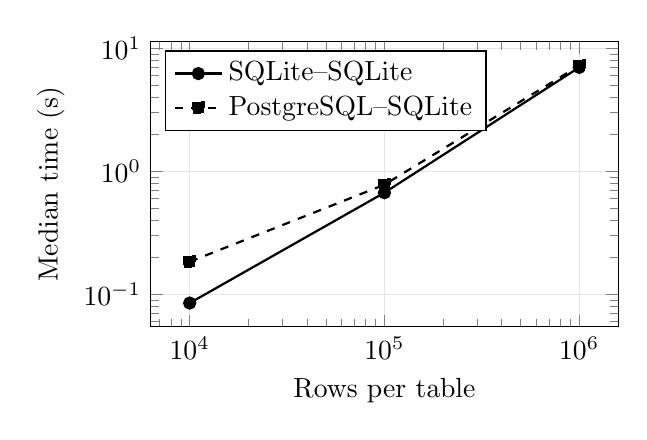
\begin{tikzpicture}
\begin{loglogaxis}[
  width=0.62\linewidth, height=5.2cm,
  xlabel={Rows per table}, ylabel={Median time (s)},
  legend pos=north west, legend cell align=left,
  grid=major, grid style={black!10}]
\addplot[mark=*, thick] coordinates {(10000,0.085) (100000,0.670) (1000000,6.982)};
\addlegendentry{SQLite--SQLite}
\addplot[mark=square*, thick, dashed] coordinates {(10000,0.184) (100000,0.778) (1000000,7.214)};
\addlegendentry{PostgreSQL--SQLite}
\end{loglogaxis}
\end{tikzpicture}
\caption{Comparison time scales linearly with table size; the cross-engine
pair converges to the single-engine cost as size grows.}
\label{fig:perf}
\end{figure}

\section{Limitations and future work}

Memory is proportional to the source table, so tables of hundreds of
millions of rows should currently be filtered or compared in key ranges. A
natural extension is to partition the key space and compare partitions
independently, which would bound memory and permit parallelism; pushing
per-partition checksums into the database, as \texttt{data-diff} did,
would further reduce data transfer when few rows differ. Views, triggers,
stored procedures and check constraints are not yet compared, and float
tolerance is absolute rather than relative. Finally, the broader framework
of \citet{rai2026universal} also covers non-relational stores such as
document databases; extending \texttt{dbcomparer} with adapters for those
backends is planned.

\section{Availability}

\texttt{dbcomparer} is released under the MIT licence. Source code,
documentation, tests and the benchmark script are at
\url{https://github.com/rairs/dbcomparer}; version 0.1.0 is archived at
\href{https://doi.org/10.5281/zenodo.24213702}{doi:10.5281/zenodo.24213702}
\citep{dbcomparer_zenodo}. It can be installed with
\texttt{pip install}\ \url{git+https://github.com/rairs/dbcomparer}, with optional
extras for PostgreSQL, MySQL, SQL Server and DuckDB drivers.

\section*{Acknowledgements}

This work received no external funding. The author thanks the maintainers
of SQLAlchemy and of the open-source database drivers used in testing.
Generative AI (Claude, Anthropic) assisted in drafting parts of the source
code, tests and manuscript text; the author reviewed, tested and edited all
such output and is responsible for the content.

\bibliographystyle{plainnat}
\bibliography{refs}

\end{document}
